\section{Introduction}
A long-term goal of robotics research is the introduction of
intelligent household robots.  To be effective, such robots will need
to perform complex tasks over long horizons (e.g., setting a dinner
table, doing laundry). Planning for these long-horizon tasks is
infeasible for state-of-the-art motion planners, making the need for a
hierarchical system of reasoning apparent.

One way to approach hierarchical planning is through combined
\emph{task and motion planning} (TAMP). In this approach, an agent is
given a symbolic, logical characterization of actions (e.g., move,
grasp, putdown), along with a geometric encoding of the
environment. TAMP systems maintain a hierarchical separation of
high-level, symbolic task planning and low-level, geometric motion
planning.  Efficient integration of these two types of reasoning is
difficult, and recent research has proposed several methods for
it~\cite{srivastava2014combined, kaelbling2011hierarchical,
  lagriffoul2014orientation, GarrettWAFR14, dornhege2012semantic}.
We adopt the principles of abstraction in the TAMP system developed by
Srivastava et al.~\cite{srivastava2014combined} (henceforth referred
to as SFRCRA-14) to factor the reasoning and search problems into
interacting logic-based and geometric components.

\begin{figure}[t]
  \centering
    \noindent
    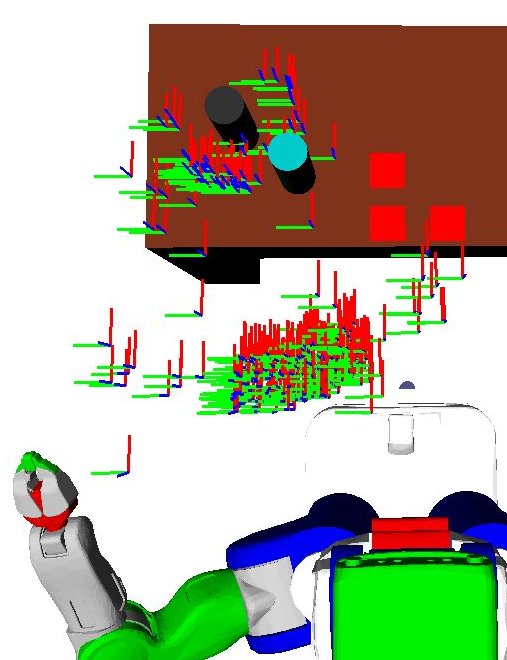
\includegraphics[scale=0.15]{images/move_grasp.png}\hspace{5 mm}
    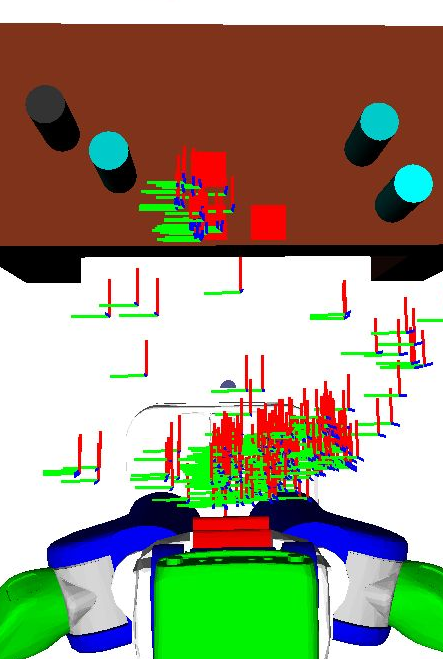
\includegraphics[scale=0.15]{images/move_putdown.png}
  \caption{\small{Screenshots showing distributions learned by our
      system in a simulated pick-and-place domain. We use
      reinforcement learning to train good sampling distributions for
      continuous motion planning parameters in long-horizon tasks. The
      robot must grasp the black can and put it down on the red
      square. The left image shows learned base position (blue) and
      grasping (green) distributions, and the right shows learned base
      position (blue) and putdown (green) distributions. The grasping
      policy learned to avoid the obstructions.}}
  \label{fig:cover}
\end{figure}

In this work, we develop a complete algorithm for TAMP and propose
methods for carrying out guided search in the space of
high-level (logic-based) plans and their low-level
\emph{refinements}, or instantiations of continuous values for
symbolic references in the plan.

In particular, we introduce
a \emph{plan refinement graph}, which allows interleaving plan
refinement (the search for symbolic reference instantiations of a plan) with a
search over \emph{which} high-level plan to try refining, given options
that address different infeasibilities. Furthermore, we present
machine learning techniques to train heuristic functions that guide
both of these search processes, making them more efficient than previous
hand-coded approaches. For example, the TAMP systems cited above use hand-coded heuristics to
search for instantiations of symbolic references, relying
on domain-specific insight from the user to reduce the space of possible values.

To learn efficient plan refinement strategies, we train distributions
to propose continuous values for symbolic references that are likely to yield
successful trajectories using a motion planner. We train these distributions through an
application of reinforcement learning (RL). Our approach draws inspiration
from Zhang and Dietterich~\cite{JobShopSched}, who applied RL to job
shop scheduling. In their formulation, states correspond to schedules
and actions propose changes to the schedule. In our setting, states
correspond to (potentially infeasible) refinements and actions propose
new values for symbolic references. We implement our approach using methods
adapted from Zucker et al.~\cite{workspacebias}, who train a
configuration space sampler for a randomized motion planner.

The contributions of our work are as follows: 1) we present a complete
algorithm for TAMP by maintaining a plan refinement graph; 2) we
present a local search algorithm for plan refinement that is easily
formulated as an MDP; 3) we formulate plan refinement in the RL
framework and learn a policy for this MDP; 4) we train heuristics to
search intelligently through a plan refinement graph; and 5) we
present experiments to evaluate our approach in a variety of simulated
domains. Our results demonstrate that our approach yields
significantly improved performance over that of SFRCRA-14.
